\section{Valores absolutos e valores relativos}
    O decibel é o resultado de uma relação logaritma entre a potência que entra em um sistema e a potência que sai do mesmo. Se o valor resultante for positivo, significa que o sinal de saída é maior que o sinal de entrada, o que representa um ganho no sistema. Se o sinal de saída for negativo, significa que o sinal de entrada é maior que o sinal de saída, o que representa uma perda no sistema. \cite{embarcados}
    
    \begin{equation*}
        Ganho_{dB} = 10 \cdot \log (\frac{P_{saida}}{P_{entrada}})
    \end{equation*}
    
    O cálculo de ganho ou perda de um sistema em decibel terá como resposta um valor absoluto. Dizer que um amplificador tem ganho de 30 dB significa dizer que ele aumenta uma potência de entrada em 1000 vezes. Uma linha de transmissão que tem uma perda de 20 dB, atenua a potência de entrada em 100 vezes.
    
    Perceba que o resultado obtido (1000 vezes) independe da unidade de medida utilizada (watts). Usando as propriedades matemáticas dos logaritmos é fácil perceber que para saber em quantas vezes é o ganho ou perda de um sistema para um valor em dB.

    \begin{equation*}
        X_{(vezes)} = 10^{(\frac{dB}{10})}
    \end{equation*}
    
    \begin{figure}[ht]
        \centering
        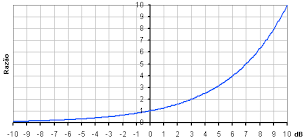
\includegraphics{db_razaop.png}
        \caption{Relação dB x Razão de potência. (Flávio Archangelo, 2011)}
    \end{figure}
    
    \newpage
    Na eletrônica pode ser conveniente relacionar o decibel a uma referência. O valor a ser encontrado será relativo à unidade de medida usada como referência. Um exemplo é a unidade dBm. Ela representa a medida de potências em relação a 1 mW. Assim, pode-se converter valores de watts para dBm. Esta medida não representa o ganho ou a perda de um sistema, e sim um valor de potência que é emitido ou recebido por um equipamento.
    
    \begin{equation*}
        \text{Potência}_{(dBm)} = 10 \cdot \log (\frac{P_{W}}{0,001W})
    \end{equation*}
